\documentclass[10.5pt]{article}
\usepackage{amsmath,amssymb,amsthm}
\usepackage{listings}
\usepackage{graphicx}
\usepackage[shortlabels]{enumitem}
\usepackage{tikz}
\usepackage[margin=1in]{geometry}
\usepackage{fancyhdr}
\usepackage{epsfig} %% for loading postscript figures
\usepackage{amsmath}
\usepackage{float}
\usepackage{amssymb}
\usepackage{caption}
\usepackage{subfigure}
\usepackage{graphics}
\usepackage{titlesec}
\usepackage{mathrsfs}
\usepackage{amsfonts}
\usepackage{indentfirst}
\usepackage{fontspec}
\usepackage{xcolor}
\renewcommand{\baselinestretch}{1.2}%Adjust Line Spacing
%\geometry{left=2.0cm,right=2.0cm,top=2.0cm,bottom=2.0cm}% Adjust Margins of the File
\usepackage{tikz-qtree}
\usetikzlibrary{graphs}
\tikzset{every tree node/.style={minimum width=2em,draw,circle},
    blank/.style={draw=none},
    edge from parent/.style=
    {draw,edge from parent path={(\tikzparentnode) -- (\tikzchildnode)}},
    level distance=1.2cm}
\setlength{\parindent}{0pt}
%\setlength{\parskip}{5pt plus 1pt}
\setlength{\headheight}{13.6pt}
\newcommand\question[2]{\vspace{.25in}\hrule\textbf{#1: #2}\vspace{.5em}\hrule\vspace{.10in}}
\renewcommand\part[1]{\vspace{.10in}\textbf{(#1)}}
\newcommand\algorithm{\vspace{.10in}\textbf{Algorithm: }}
\newcommand\correctness{\vspace{.10in}\textbf{Correctness: }}
\newcommand\runtime{\vspace{.10in}\textbf{Running time: }}
\pagestyle{fancyplain}
% Create horizontal rule command with an argument of height
\newcommand{\horrule}[1]{\rule{\linewidth}{#1}}
% Set the title here
\title{
    \normalfont \normalsize
    \textsc{ShanghaiTech University} \\ [25pt]
    \horrule{0.5pt} \\[0.4cm] % Thin top horizontal rule
    \huge CS101 Algorithms and Data Structures\\ % The assignment title
    \LARGE Fall 2020\\
    \LARGE Homework 6\\
    \horrule{2pt} \\[0.5cm] % Thick bottom horizontal rule
}
% wrong usage of \author, never mind
\author{}
\date{Due date: 23:59, September 26, 2019}

% set the header and footer
\pagestyle{fancy}
\lhead{CS101 Algorithms and Data Structures}
\chead{Homework 6}
\rhead{Due date: 23:59, October 26, 2019}
\cfoot{\thepage}
\renewcommand{\headrulewidth}{0.4pt}

% special settings for the first page
\fancypagestyle{firstpage}
{
    \renewcommand{\headrulewidth}{0pt}
    \fancyhf{}
    \fancyfoot[C]{\thepage}
}

% Add the support for auto numbering
% use \problem{title} or \problem[number]{title} to add a new problem
% also \subproblem is supported, just use it like \subsection
\newcounter{ProblemCounter}
\newcounter{oldvalue}
\newcommand{\problem}[2][-1]{
    \setcounter{oldvalue}{\value{secnumdepth}}
    \setcounter{secnumdepth}{0}
    \ifnum#1>-1
        \setcounter{ProblemCounter}{0}
    \else
        \stepcounter{ProblemCounter}
    \fi
    \section{Problem \arabic{ProblemCounter}: #2}
    \setcounter{secnumdepth}{\value{oldvalue}}
}
\newcommand{\subproblem}[1]{
    \setcounter{oldvalue}{\value{section}}
    \setcounter{section}{\value{ProblemCounter}}
    \subsection{#1}
    \setcounter{section}{\value{oldvalue}}
}

\setmonofont{Consolas}
\definecolor{blve}{rgb}{0.3372549 , 0.61176471, 0.83921569}
\definecolor{gr33n}{rgb}{0.29019608, 0.7372549 , 0.64705882}
\makeatletter
\lst@InstallKeywords k{class}{classstyle}\slshape{classstyle}{}ld
\makeatother
\lstset{language=C++,
        basicstyle=\ttfamily,
        keywordstyle=\color{blve}\ttfamily,
        stringstyle=\color{red}\ttfamily,
        commentstyle=\color{green}\ttfamily,
        morecomment=[l][\color{magenta}]{\#},
        classstyle = \bfseries\color{gr33n}, 
        tabsize=4
}


\begin{document}

\maketitle
\thispagestyle{firstpage}
%\newpage
\vspace{3ex}

\begin{enumerate}
\item Please write your solutions in English. 

\item Submit your solutions to gradescope.com.  

\item Set your FULL Name to your Chinese name and your STUDENT ID correctly in Account Settings. 

\item If you want to submit a handwritten version, scan it clearly. Camscanner is recommended. 

\item When submitting, match your solutions to the according problem numbers correctly. 

\item No late submission will be accepted.

\item Violations to any of the above may result in zero grade. 
\end{enumerate}
\newpage


%---------------------------------------------------------------
\problem{Multiple Choices}
Multiple Choices: Each question has one or more correct answer(s). Select all the correct answer(s). For each question, you get $0$ point if you select one or more wrong answers, but you get half points if you select a non-empty subset of the correct answers.\\
\textit{Note that you should write you answers of Problem 1 in the table below.}
\begin{table}[htbp]
\begin{tabular}{|p{1.5cm}|p{1.5cm}|p{1.5cm}|}
\hline 
Q(1) & Q(2) & Q(3) \\
\hline 
&&\\ 
\hline 
\end{tabular} 
\end{table} \\
%%%%% (1)
(1) Which of the following statements about the binary tree and the heap is true? \\
A. If the in-order traversal and post-order traversal of two binary trees are equal respectively, then the two binary trees are exactly the same. \\
B. If the pre-order traversal and post-order traversal of two binary trees are equal respectively, then the two binary trees are exactly the same. \\
C. If the post-order traversal of a complete binary tree is descending, then the binary tree is a min-heap. \\
D. If a binary tree is a min-heap, then the post-order traversal of this tree is descending.\\

~\\
%%%%% (2)
(2) Which traversals of binary tree 1 and binary tree 2, will produce the same sequence node name?\\
\begin{minipage}{1\textwidth}
\centering
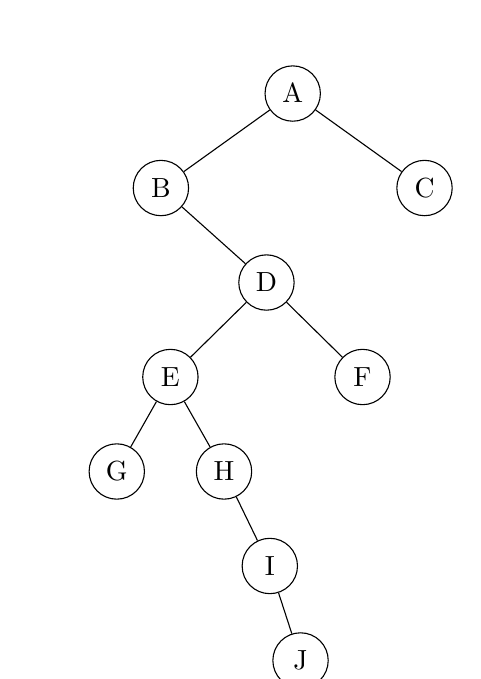
\begin{tikzpicture}
\Tree
[.A
    [.B
        \edge[blank]; \node[blank]{};
        \edge[];[.D
            \edge[];[.E
                \edge[];[.G ]
                \edge[];[.H
                    \edge[blank]; \node[blank]{};
                    \edge[];[.I 
                        \edge[blank]; \node[blank]{};
                        \edge[];[.J
                        ] 
                    ]
                ]
            ]
            \edge[]; [.F
            ]
        ]
    ]
    [.C
    ]
]
\end{tikzpicture}
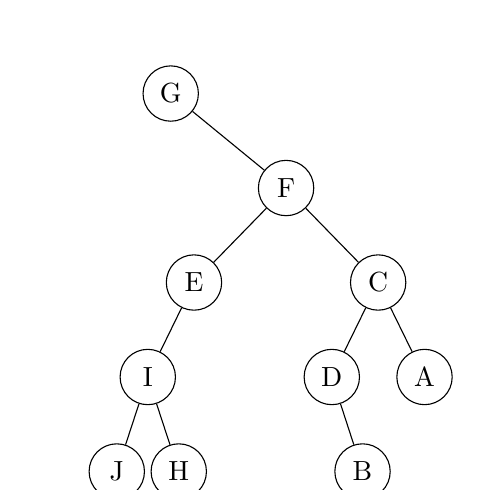
\begin{tikzpicture}
\Tree
[.G
    \edge[blank]; \node[blank]{};
    \edge[]; [.F
        \edge[]; [.E 
            \edge[];[.I 
                \edge[];[.J ]
                \edge[];[.H ]
            ]
            \edge[blank]; \node[blank]{};
        ]
        \edge[]; [.C 
            \edge[]; [.D
                \edge[blank]; \node[blank]{};
                \edge[];[.B ]  
            ]
            \edge[]; [.A ]
        ] 
    ]
]
\end{tikzpicture}
\end{minipage} \\
A. Post-order, Post-order \\
B. Post-order, In-order \\
C. In-order, In-order \\
D. Pre-order, Pre-order \\
~\\

%%%%% (2)
(3) Which of the following statements about the binary heap is \textbf{not} true? \\
A. There exists a heap with seven distinct elements so that the in-order traversal gives the element in sorted order. \\
B. If item A is an ancestor of item B in a heap (used as a Priority Queue) then it must be the case that the Insert operation for item A occurred before the \textbf{Insert} operation for item B.\\
C. If array A is sorted from smallest to largest then A (excluding A[0]) corresponds to a min-heap. \\
D. None of the above. \\
~\\

% -------------------------------------------------------------------------
\problem{Construct a Heap}
(1) Suppose we construct a min-heap from the following array: ${120,140,40,50,80,70,60,90,20,100}$, by inserting elements into a empty heap in sequence. After the construction is completed, what should this heap look like? Please draw it as a binary tree.\\
\vspace{150}

(2) Suppose we construct a min-heap from the following initial heap by Floyd's method. After the construction is completed, we delete the root from the heap. What will be the post-order traversal of the heap? Write down your answer in the table above directly.\\
Your answer: \underline{\hspace{300}}.\\

\begin{minipage}{1\textwidth}
\centering
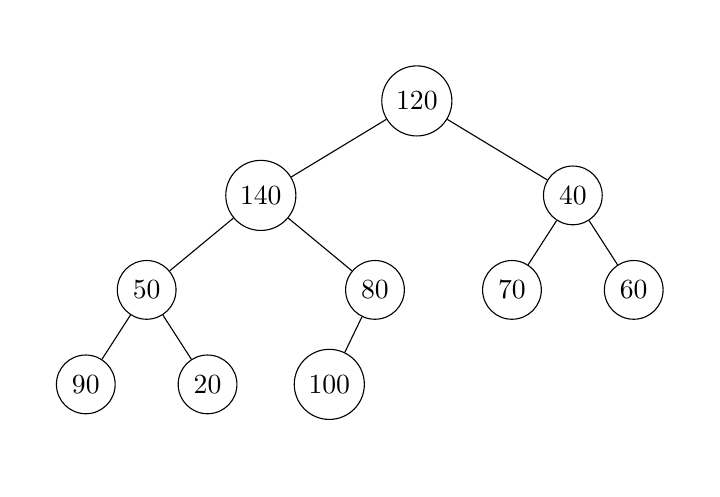
\begin{tikzpicture}
\Tree
[.120
[.140
\edge[]; [.50
\edge[]; [.90
\edge[blank]; \node[blank]{};
\edge[blank]; \node[blank]{};
]
\edge[]; [.20
\edge[blank]; \node[blank]{};
\edge[blank]; \node[blank]{};
]
]
\edge[]; [.80
\edge[]; [.100
\edge[blank]; \node[blank]{};
\edge[blank]; \node[blank]{};
]
\edge[blank]; \node[blank]{};
]
]
[.40
% \edge[blank]; \node[blank]{};
\edge[]; [.70
\edge[blank]; \node[blank]{};
\edge[blank]; \node[blank]{};
]
\edge[]; [.60
\edge[blank]; \node[blank]{};
\edge[blank]; \node[blank]{};
]
]
]
\end{tikzpicture}
\end{minipage}%

(3) If we use the Floyd's method to build a heap of size $N$, the worst-case time complexity is \underline{\hspace{50}}.\\
(4) If we use the "inserting elements into a empty heap" method to build a heap of size $N$, the worst-case time complexity is \underline{\hspace{50}}.\\

\pagebreak

%------------------------------------------------------------------
\problem{Heap Sort}
\paragraph{}
You are given such a max heap like this:

\begin{minipage}{1\textwidth}
\centering
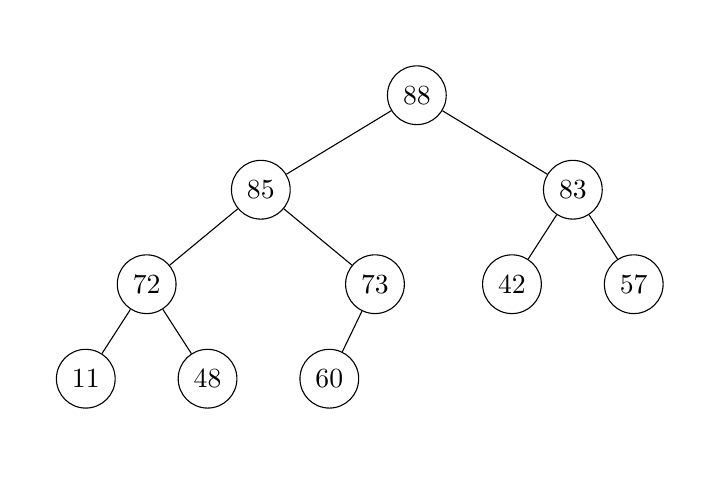
\begin{tikzpicture}
\Tree
[.88
    [.85
        \edge[]; [.72
            \edge[]; [.11
                \edge[blank]; \node[blank]{};
                \edge[blank]; \node[blank]{};
            ]
            \edge[]; [.48
                \edge[blank]; \node[blank]{};
                \edge[blank]; \node[blank]{};
            ]
        ]
        \edge[]; [.73
            \edge[]; [.60
                \edge[blank]; \node[blank]{};
                \edge[blank]; \node[blank]{};
            ]
            \edge[blank]; \node[blank]{};
        ]
    ]
    [.83
    % \edge[blank]; \node[blank]{};
        \edge[]; [.42
            \edge[blank]; \node[blank]{};
            \edge[blank]; \node[blank]{};
        ]
        \edge[]; [.57
            \edge[blank]; \node[blank]{};
            \edge[blank]; \node[blank]{};
        ]
    ]
]
\end{tikzpicture}
\end{minipage}%

Then you need to use array method to show each step of heap sort in increasing order. Fill in the value in the table below. Notice that the value we have put is the step of each value sorted successfully. For each step, you should always make you heap satisfies the requirement of max heap property.

\begin{table}[!hbtp]
\centering
\resizebox{\textwidth}{!}{%
    \begin{tabular}{|c|c|c|c|c|c|c|c|c|c|c|c|}
        \hline
        index & 0 & 1 & 2 & 3 & 4 & 5 & 6 & 7 & 8 & 9 & 10 \\ \hline
        value & $\quad $ & $\quad $ & $\quad $ &$\quad $  &$\quad $  & $\quad $ &$\quad $  &$\quad $  & $\quad $ &$\quad $  &$\quad $  \\ \hline
    \end{tabular}%
}
\caption{The original array to represent max heap.}
\label{}
\end{table}
\begin{table}[!hbtp]
\centering
\resizebox{\textwidth}{!}{%
    \begin{tabular}{|c|c|c|c|c|c|c|c|c|c|c|c|}
        \hline
        index & 0 & 1 & 2 & 3 & 4 & 5 & 6 & 7 & 8 & 9 & 10 \\ \hline
        value & $\quad $ &$\quad $  &$\quad $  &$\quad $  &$\quad $  & $\quad $ &$\quad $  &$\quad $  &$\quad $  &$\quad $  & \color{blue}88 \\ \hline
    \end{tabular}%
}
\caption{First value is successfully sorted.}
\label{}
\end{table}
\begin{table}[h]
\centering
\resizebox{\textwidth}{!}{%
    \begin{tabular}{|c|c|c|c|c|c|c|c|c|c|c|c|}
        \hline
        index & 0 & 1 & 2 & 3 & 4 & 5 & 6 & 7 & 8 & 9 & 10 \\ \hline
        value &$\quad $  &$\quad $ & $\quad $ & $\quad $ & $\quad $ & $\quad $ & $\quad $ & $\quad $& $\quad $ & \color{blue}85 & \color{blue}88 \\ \hline
    \end{tabular}%
}
\caption{Second value is successfully sorted.}
\label{}
\end{table}
\begin{table}[!hbtp]
\centering
\resizebox{\textwidth}{!}{%
    \begin{tabular}{|c|c|c|c|c|c|c|c|c|c|c|c|}
        \hline
        index & 0 & 1 & 2 & 3 & 4 & 5 & 6 & 7 & 8 & 9 & 10 \\ \hline
        value &$\quad $  & $\quad $ & $\quad $ & $\quad $ & $\quad $ & $\quad $ & $\quad $ & $\quad $ & \color{blue}83 & \color{blue}85 & \color{blue}88  \\ \hline
    \end{tabular}%
}
\caption{Third value is successfully sorted.}
\label{}
\end{table}
\begin{table}[!hbtp]
\centering
\resizebox{\textwidth}{!}{%
    \begin{tabular}{|c|c|c|c|c|c|c|c|c|c|c|c|}
        \hline
        index & 0 & 1 & 2 & 3 & 4 & 5 & 6 & 7 & 8 & 9 & 10 \\ \hline
        value &$\quad $  & $\quad $ & $\quad $ & $\quad $ & $\quad $ & $\quad $ & $\quad $ & \color{blue}73 & \color{blue}83 & \color{blue}85 & \color{blue}88 \\ \hline
    \end{tabular}%
}
\caption{Fourth value is successfully sorted.}
\label{}
\end{table}
\begin{table}[!hbtp]
\centering
\resizebox{\textwidth}{!}{%
    \begin{tabular}{|c|c|c|c|c|c|c|c|c|c|c|c|}
        \hline
        index & 0 & 1 & 2 & 3 & 4 & 5 & 6 & 7 & 8 & 9 & 10 \\ \hline
        value & $\quad $ & $\quad $ & $\quad $ & $\quad $ & $\quad $ & $\quad $ & \color{blue}72 & \color{blue}73 & \color{blue}83 & \color{blue}85 & \color{blue}88 \\ \hline
    \end{tabular}%
}
\caption{Fifth value is successfully sorted.}
\label{}
\end{table}
\begin{table}[!hbtp]
\centering
\resizebox{\textwidth}{!}{%
    \begin{tabular}{|c|c|c|c|c|c|c|c|c|c|c|c|}
        \hline
        index & 0 & 1 & 2 & 3 & 4 & 5 & 6 & 7 & 8 & 9 & 10 \\ \hline
        value & $\quad $ & $\quad $ & $\quad $& $\quad $ & $\quad $ & \color{blue}60 & \color{blue}72 & \color{blue}73 & \color{blue}83 & \color{blue}85 & \color{blue}88 \\ \hline
    \end{tabular}%
}
\caption{Sixth value is successfully sorted.}
\label{}
\end{table}
\begin{table}[!hbtp]
\centering
\resizebox{\textwidth}{!}{%
    \begin{tabular}{|c|c|c|c|c|c|c|c|c|c|c|c|}
        \hline
        index & 0 & 1 & 2 & 3 & 4 & 5 & 6 & 7 & 8 & 9 & 10 \\ \hline
        value & $\quad $ & $\quad $ & $\quad $ & $\quad $ & \color{blue}57 & \color{blue}60 & \color{blue}72 & \color{blue}73 & \color{blue}83 & \color{blue}85 & \color{blue}88 \\ \hline
    \end{tabular}%
}
\caption{Seventh value is successfully sorted.}
\label{}
\end{table}
\begin{table}[!hbtp]
\centering
\resizebox{\textwidth}{!}{%
    \begin{tabular}{|c|c|c|c|c|c|c|c|c|c|c|c|}
        \hline
        index & 0 & 1 & 2 & 3 & 4 & 5 & 6 & 7 & 8 & 9 & 10 \\ \hline
        value &$\quad $  & $\quad $ & $\quad $ & \color{blue}48 & \color{blue}57 & \color{blue}60 & \color{blue}72 & \color{blue}73 & \color{blue}83 & \color{blue}85 & \color{blue}88 \\ \hline
    \end{tabular}%
}
\caption{Eighth value is successfully sorted.}
\label{}
\end{table}
\begin{table}[!hbtp]
\centering
\resizebox{\textwidth}{!}{%
    \begin{tabular}{|c|c|c|c|c|c|c|c|c|c|c|c|}
        \hline
        index & 0 & 1 & 2 & 3 & 4 & 5 & 6 & 7 & 8 & 9 & 10 \\ \hline
        value & $\quad $ & \color{blue}11 & \color{blue}42 & \color{blue}48 & \color{blue}57 & \color{blue}60 & \color{blue}72 & \color{blue}73 & \color{blue}83 & \color{blue}85 & \color{blue}88 \\ \hline
    \end{tabular}%
}
\caption{Last 2 values are successfully sorted.}
\label{}
\end{table}
\newpage
\problem{Median Produce 101}
\paragraph{}
The well known TV show \textit{Produce 101} has a new rule to judge all the singers: for each singer, use the median score among all the judges to set her score. Previously, the program groups have a calculator to calculate the score for each singer. Accidentally, the calculator is broken one day. And the fans of singer
ChaoYue are eagerly waiting for the score. So they want to help the program group to calculate the correct median score.

Recall that the median value of a set is the value that separates the higher half of set's values from the set's values from the set's lower values. 

For example, given the set with \textbf{odd} numbers of elements:

\begin{center}
$\{78,94,17,87,65\}$
\end{center}

The median score is 78.\\

For another example, given the set with \textbf{even} numbers of elements:

\begin{center}
$\{78,94,17,87,65,76\}$
\end{center}

The median score is $(78+76)/2=77$.
\paragraph{}

Consider a set $S$ of arbitrary and distinct integer scores (not necessatily the set shown above). Let $n$ denote the size of set $S$, and assume throughtout this problem that $n$ can be odd or even.

Now, fancy fans finds a data structure "Dynamic Medians" for maintaining a set $S$ of numbers, supporting the following operations:

\textbf{CREATE():} Creat an empty set $S$

\textbf{INSERT(x):} Add a new given number $x$ to $S$

\textbf{MEDIAN():} Return a median of $S$.

Assume no duplicates are added to $S$. He proposes to implement this “dynamic median” data structure DM using a maxheap
$A$ and a minheap $B$, such that the following two properties always hold:

1. Every element in $A$ is less than every element in $B$, and

2. the size of $A$ equals the size of $B$, or is one less.

To return a median of $S$, she proposes to return the minimum element of $B$.

\newpage
(1) Argue that this is correct (i.e., that a median is returned)


\newpage
(2) Explain how to implement \textbf{INSERT(x)}, while maintaining the relevant properties.
Analyze the most efficient running time of \textbf{INSERT} algorithm in terms of $n$, the number
of elements in $S$.

\end{document}